\documentclass[aspectratio=169, 10pt]{beamer}

% Load Preamble
% Course Slide Deck Preamble
\usepackage[utf8]{inputenc}
\usepackage{amsmath,amssymb,amsfonts}
\usepackage{graphicx}
\usepackage{xcolor}
\usepackage{listings}
\usepackage{booktabs}
\usepackage{tikz}
\usetikzlibrary{positioning, calc, shadows, fit, arrows.meta, decorations.pathreplacing, backgrounds}

% Color Palette
\definecolor{mainblue}{RGB}{24, 76, 120}
\definecolor{accentblue}{RGB}{0, 136, 204}
\definecolor{codebg}{RGB}{245, 247, 250}
\definecolor{codeframe}{RGB}{200, 205, 215}
\definecolor{commentgreen}{RGB}{46, 139, 87}
\definecolor{keywordpurple}{RGB}{128, 0, 128}
\definecolor{stringred}{RGB}{178, 34, 34}
\definecolor{shadowgray}{RGB}{220, 224, 230}

% Beamer Theme Base
\usetheme{Madrid}
\usecolortheme{whale}

% White Title Header with Black Text
\setbeamercolor{frametitle}{bg=white,fg=black}
\setbeamercolor{titlelike}{bg=white,fg=black}
\setbeamercolor{structure}{fg=mainblue}
\setbeamercolor{palette primary}{bg=mainblue,fg=white}
\setbeamercolor{palette secondary}{bg=accentblue,fg=white}

% Remove navigation symbols & Clean Footline
\setbeamertemplate{navigation symbols}{}
\setbeamertemplate{footline}{%
    \begin{beamercolorbox}[wd=\paperwidth,ht=0.4cm,dp=0.15cm,leftskip=0.8cm,rightskip=0.8cm]{footline}%
        {\fontsize{7pt}{8pt}\selectfont \color{gray} Prof. Artur Yakimovich. MLID. CC BY 4.0 (2026)}%
        \hfill%
        {\fontsize{7pt}{8pt}\selectfont \color{gray} \insertframenumber{} / \inserttotalframenumber}%
    \end{beamercolorbox}%
}

% Custom Frame Title with Vertically Centered Title & Logo + Drop Shadow Line
\setbeamertemplate{frametitle}{
    \nointerlineskip
    \begin{beamercolorbox}[wd=\paperwidth,ht=1.2cm,dp=0cm]{frametitle}
        \begin{tikzpicture}
            \useasboundingbox (0,0) rectangle (\paperwidth,1.2cm);
            \node[anchor=west, inner sep=0pt, align=left] at (0.8cm, 0.6cm) {%
                \begin{minipage}{0.70\paperwidth}
                    \raggedright
                    {\usebeamerfont{frametitle}\color{black}\insertframetitle\par}%
                    \ifx\insertframesubtitle\@empty
                    \else
                        \vspace{1pt}%
                        {\usebeamerfont{framesubtitle}\color{gray}\insertframesubtitle\par}%
                    \fi
                \end{minipage}%
            };
            \node[anchor=east, inner sep=0pt] at (\paperwidth-0.8cm, 0.6cm) {%
                
\includegraphics[height=0.7cm,keepaspectratio]{../assets/logo.png}%
            };
        \end{tikzpicture}%
    \end{beamercolorbox}
    % Soft gray drop shadow / line separator
    \nointerlineskip
    \vspace{-1pt}
    
\begin{tikzpicture}[remember picture, overlay]
        \fill[shadowgray] (0,0) rectangle (\paperwidth, -0.04cm);
        \fill[gray!20, opacity=0.5] (0,-0.04cm) rectangle (\paperwidth, -0.08cm);
    \end{tikzpicture}
}

% Listings Configuration for Python Code
\lstset{
    language=Python,
    backgroundcolor=\color{codebg},
    basicstyle=\ttfamily\fontsize{6.5pt}{7.5pt}\selectfont\color{black},
    keywordstyle=\bfseries\color{keywordpurple},
    commentstyle=\itshape\color{commentgreen},
    stringstyle=\color{stringred},
    numbers=none,
    breaklines=true,
    showstringspaces=false,
    tabsize=2,
    frame=single,
    rulecolor=\color{codeframe}
}

% Custom Commands
\newcommand{\E}{\mathbb{E}}
\newcommand{\R}{\mathbb{R}}
\newcommand{\KL}[2]{D_{\text{KL}}\left(#1 \,||\, #2\right)}
\newcommand{\Lsimple}{\mathcal{L}_{\text{simple}}}


\title[GenAI Bioimage Analysis]{Bridging Scales through Generative AI for Inverse Problems in Biomedical Computational Microscopy}
\subtitle{Mathematical Concepts, Inverse Problems, \& VIRVS Virtual Staining Benchmark}
\author{Prof. Artur Yakimovich. Machine Learning for Infection and Disease Group}
\institute{\vspace{0.2cm}\fontsize{7pt}{8pt}\selectfont \textbf{License}: Licensed under Creative Commons Attribution 4.0 International (\textbf{CC BY 4.0})}
\date{\today}

\begin{document}

% Title Slide
\begin{frame}[plain]
    \titlepage
    \vspace{-0.5cm}
    \centering
    
\includegraphics[height=1.0cm]{../assets/logo.png}
\end{frame}

% Table of Contents Slide
\begin{frame}{Course Overview}
    \tableofcontents
\end{frame}

% Include Section Slides
% Section 1: Introduction to Inverse Problems & Virtual Staining

\section{Inverse Problems in Bioimaging}

\begin{frame}[fragile]{Optical Physics: Microscope PSF Formation}
    \begin{columns}
        \column{0.48\textwidth}
        \textbf{Physics of Impulse Response}

        \begin{itemize}
            \item \textbf{Point Source}: A fluorophore emits spherical wavefronts $\delta(x,y)$.
            \item \textbf{Finite Aperture}: Objective lens with numerical aperture $\text{NA} = n \sin \alpha$ caps high spatial frequencies (low-pass filter).
            \item \textbf{Point Spread Function (PSF)}: Diffraction transforms a point source into an Airy pattern $h(r) \propto \left(\frac{J_1(k r)}{k r}\right)^2$.
            \item \textbf{Abbe Limit}: Minimum resolvable distance $d = \frac{\lambda}{2\text{NA}}$.
        \end{itemize}

        \vspace{1mm}
        \textbf{\color{commentgreen}Biological Intuition (DAPI $\to$ GFP):}\\
        \fontsize{6.5pt}{7.5pt}\selectfont
        Single GFP fluorophores or fine DAPI chromatin granules are physically blurred by the microscope's PSF into smooth Airy disks. Generative models act as non-linear deconvolution solvers.

        \column{0.52\textwidth}
        \textbf{Microscope Optics \& Code}

        \centering
        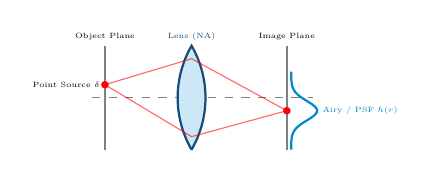
\begin{tikzpicture}[scale=0.55, every node/.style={transform shape}]
            % Axis
            \draw[dashed, gray] (-0.3,0) -- (4.8,0);
            % Object Plane
            \draw[thick, gray] (0,-1.2) -- (0,1.2) node[above, black] {\tiny Object Plane};
            \fill[red] (0,0.3) circle (2.5pt) node[left, black] {\tiny Point Source $\delta$};
            % Lens
            \draw[thick, mainblue, fill=accentblue!20] (2.0,-1.2) arc (-30:30:2.4) arc (150:210:2.4);
            \node[above, mainblue] at (2.0,1.2) {\tiny Lens (NA)};
            % Rays
            \draw[red, opacity=0.6] (0,0.3) -- (2.0,0.9) -- (4.2,-0.3);
            \draw[red, opacity=0.6] (0,0.3) -- (2.0,-0.9) -- (4.2,-0.3);
            % Image Plane & PSF Profile
            \draw[thick, gray] (4.2,-1.2) -- (4.2,1.2) node[above, black] {\tiny Image Plane};
            \fill[red] (4.2,-0.3) circle (2.5pt);
            \draw[smooth, domain=-0.9:0.9, variable=\y, color=accentblue, thick]
            plot ({4.3 + 0.6*exp(-10*(\y)^2)}, {\y - 0.3});
            \node[right, accentblue] at (4.9,-0.3) {\tiny Airy / PSF $h(r)$};
        \end{tikzpicture}

        \begin{lstlisting}
import torch

def generate_2d_gaussian_psf(size=15, sigma=2.0):
    # Coordinate grid
    coords = torch.arange(size) - size // 2
    y, x = torch.meshgrid(coords, coords, indexing='ij')
    
    # 2D Gaussian PSF approximation h(r)
    r_sq = x**2 + y**2
    psf = torch.exp(-r_sq / (2 * sigma**2))
    psf = psf / psf.sum() # Normalize integral to 1
    return psf.unsqueeze(0).unsqueeze(0)
\end{lstlisting}
    \end{columns}
\end{frame}

\begin{frame}[fragile]{Forward Problems in Bioimage Acquisition}
    \begin{columns}
        \column{0.48\textwidth}
        \textbf{Mathematical Formulation}

        Microscope image formation is a \textbf{forward problem}:
        \begin{equation*}
            y = A(x) + n
        \end{equation*}

        \begin{itemize}
            \item $x \in \R^N$: True biological signal (GFP reporter).
            \item $A$: Optical degradation (PSF blur, phase).
            \item $n \sim \mathcal{N}(0, \sigma^2 I)$: Detector noise.
            \item $y \in \R^M$: Observed micrograph (DAPI stain).
        \end{itemize}

        \vspace{1mm}
        \textbf{\color{commentgreen}Biological Intuition (DAPI $\to$ GFP):}\\
        \fontsize{6.5pt}{7.5pt}\selectfont
        DAPI ($y$) reveals nuclear boundaries and chromatin texture, which are optical projections of cell state. GFP ($x$) marks positive expression. Microscope optics blur and add noise to these signals.

        \column{0.52\textwidth}
        \textbf{Python Code Equivalent}
        \begin{lstlisting}
import torch
import torch.nn.functional as F

def forward_observation(x, psf, sigma=0.05):
    # Blur image with Point Spread Function
    blurred = F.conv2d(x, psf, padding=1)
    
    # Add Gaussian detector noise n ~ N(0, sigma^2)
    noise = torch.randn_like(blurred) * sigma
    
    y = blurred + noise
    return y
\end{lstlisting}
    \end{columns}
\end{frame}


\begin{frame}[fragile]{Ill-Posedness of the Inverse Problem}
    \begin{columns}
        \column{0.48\textwidth}
        \textbf{Mathematical Formulation}

        Reconstructing $x$ from $y$ requires solving the \textbf{inverse problem}:
        \begin{equation*}
            \hat{x} = A^{\dagger} y
        \end{equation*}

        Hadamard criteria for well-posedness:
        \begin{enumerate}
            \item \textbf{Existence}: Solution exists.
            \item \textbf{Uniqueness}: Unique solution.
            \item \textbf{Stability}: Continuous dependence on data $y$.
        \end{enumerate}

        Bioimaging inverse problems are \textbf{severely ill-posed}: $A$ is non-invertible/lossy!

        \vspace{1mm}
        \textbf{\color{commentgreen}Biological Intuition (DAPI $\to$ GFP):}\\
        \fontsize{6.5pt}{7.5pt}\selectfont
        Multiple cells may have identical nuclear shapes in DAPI, but some are GFP-positive and others negative. Inverting nuclear stain alone is ill-posed without spatial priors.

        \column{0.52\textwidth}
        \textbf{Python Code Equivalent}
        \begin{lstlisting}
# Naive inversion fails due to noise amplification

def naive_inversion(y, A_matrix):
    # SVD decomposition of measurement operator
    u, s, vh = torch.linalg.svd(A_matrix)
    
    # Small singular values amplify noise
    s_inv = torch.where(s > 1e-4, 1.0 / s, 0.0)
    A_pinv = vh.T @ torch.diag(s_inv) @ u.T
    
    x_hat = A_pinv @ y
    return x_hat
\end{lstlisting}
    \end{columns}
\end{frame}


\begin{frame}[fragile]{Classical Regularization (Tikhonov / Ridge)}
    \begin{columns}
        \column{0.48\textwidth}
        \textbf{Mathematical Formulation}

        To stabilize ill-posed inverse problems, we penalize implausible solutions:
        \begin{equation*}
            \hat{x} = \arg\min_x \|y - Ax\|_2^2 + \lambda \|x\|_2^2
        \end{equation*}

        Closed-form solution:
        \begin{equation*}
            \hat{x} = (A^T A + \lambda I)^{-1} A^T y
        \end{equation*}

        \begin{itemize}
            \item First term: Data fidelity (observed $y$).
            \item Second term: Prior/regularizer ($L_2$ norm).
            \item $\lambda > 0$: Regularization strength.
        \end{itemize}

        \vspace{1mm}
        \textbf{\color{commentgreen}Biological Intuition (DAPI $\to$ GFP):}\\
        \fontsize{6.5pt}{7.5pt}\selectfont
        Penalizes unrealistically extreme GFP intensity spikes outside cell boundaries, enforcing a smooth prior that fluorescence shouldn't explode randomly.

        \column{0.52\textwidth}
        \textbf{Python Code Equivalent}
        \begin{lstlisting}
def tikhonov_reconstruction(y, A, lmbda=1e-2):
    # A: [M, N] measurement matrix
    # y: [M, 1] observation vector
    N = A.shape[1]
    
    # System: (A^T A + lambda * I) x = A^T y
    AtA = A.T @ A
    regularizer = lmbda * torch.eye(N, device=A.device)
    
    lhs = AtA + regularizer
    rhs = A.T @ y
    
    x_hat = torch.linalg.solve(lhs, rhs)
    return x_hat
\end{lstlisting}
    \end{columns}
\end{frame}


\begin{frame}[fragile]{Autoencoders (AEs) \& Representation Learning}
    \begin{columns}
        \column{0.48\textwidth}
        \textbf{Mathematical Formulation}

        Compression into a low-dimensional bottleneck $z \in \R^d$ ($d \ll N$):
        \begin{align*}
            z &= e_\phi(x) \quad \text{(Encoder)} \\
            \hat{x} &= d_\theta(z) \quad \text{(Decoder)}
        \end{align*}
        Reconstruction Loss: $\mathcal{L}_{\text{AE}} = \|x - d_\theta(e_\phi(x))\|_2^2$

        \textbf{Generative Sampling Limitation}:
        Deterministic $z$-space has gaps and unconstrained regions. Random sampling $z \sim \mathcal{N}(0, I)$ produces unrealistic artifacts!

        \vspace{1mm}
        \textbf{\color{commentgreen}Biological Intuition (DAPI $\to$ GFP):}\\
        \fontsize{6.5pt}{7.5pt}\selectfont
        Standard AE compresses DAPI nuclear shape and GFP expression into bottleneck $z$. But because $z$-space has gaps, sampling random vectors yields non-biological cell artifacts.

        \column{0.52\textwidth}
        \textbf{Python Code Equivalent}
        \begin{lstlisting}
import torch.nn as nn

class Autoencoder(nn.Module):
    def __init__(self, latent_dim=32):
        super().__init__()
        self.encoder = nn.Sequential(
            nn.Conv2d(1, 16, 3, stride=2, padding=1),
            nn.ReLU(),
            nn.Flatten(),
            nn.Linear(16 * 128 * 128, latent_dim)
        )
        self.decoder = nn.Sequential(
            nn.Linear(latent_dim, 16 * 128 * 128),
            nn.Unflatten(1, (16, 128, 128)),
            nn.ConvTranspose2d(16, 1, 3, stride=2, padding=1, output_padding=1),
            nn.Sigmoid()
        )

    def forward(self, x):
        z = self.encoder(x)
        return self.decoder(z)
\end{lstlisting}
    \end{columns}
\end{frame}


\begin{frame}[fragile]{Variational Autoencoders \& Generative Sampling}
    \begin{columns}
        \column{0.48\textwidth}
        \textbf{Mathematical Formulation}

        Map input $x$ to latent distribution parameters $(\mu_\phi(x), \sigma_\phi(x))$:
        \begin{equation*}
            z = \mu_\phi(x) + \sigma_\phi(x) \odot \epsilon, \quad \epsilon \sim \mathcal{N}(0, I)
        \end{equation*}
        Objective (ELBO):
        \begin{equation*}
            \mathcal{L}_{\text{VAE}} = \|x - \hat{x}\|_2^2 + \beta \, \KL{q_\phi(z|x)}{\mathcal{N}(0, I)}
        \end{equation*}

        \textbf{Generative Sampling}:
        $\text{KL}$ penalty regularizes $z$-space to be smooth and gap-free. We can synthesize NEW valid cell images by sampling $z \sim \mathcal{N}(0, I)$!

        \vspace{1mm}
        \textbf{\color{commentgreen}Biological Intuition (DAPI $\to$ GFP):}\\
        \fontsize{6.5pt}{7.5pt}\selectfont
        VAE regularizes cell latent space so nuclear features and GFP expression vary smoothly. We can sample new synthetic DAPI/GFP cells or interpolate between GFP-negative and GFP-positive states!

        \column{0.52\textwidth}
        \textbf{Python Code Equivalent}
        \begin{lstlisting}
# Generative Sampling from Trained VAE Decoder

def generate_samples(decoder, num_samples=16, latent_dim=32, device='cpu'):
    decoder.eval()
    with torch.no_grad():
        # 1. Sample z ~ N(0, I) from standard Gaussian prior
        z_random = torch.randn(num_samples, latent_dim, device=device)
        
        # 2. Decode latent vectors into synthetic cell images
        x_synthetic = decoder(z_random)
        
    return x_synthetic # [num_samples, 1, H, W]
\end{lstlisting}
    \end{columns}
\end{frame}


\begin{frame}[fragile]{Learning the Prior: Deep Inverse Problems}
    \begin{columns}
        \column{0.48\textwidth}
        \textbf{Mathematical Formulation}

        Instead of hand-crafted priors $\|x\|_2^2$ or $\text{TV}(x)$, we learn a data-driven mapping $f_\theta$:
        \begin{equation*}
            \hat{x} = f_\theta(y) \approx \arg\min_x \Big( \|y - A(x)\|^2 + \lambda R_\theta(x) \Big)
        \end{equation*}

        Empirical Risk Minimization over training pairs $(y_i, x_i)$:
        \begin{equation*}
            \theta^* = \arg\min_\theta \frac{1}{N} \sum_{i=1}^N \mathcal{L}\big( f_\theta(y_i), \, x_i \big)
        \end{equation*}

        \vspace{1mm}
        \textbf{\color{commentgreen}Biological Intuition (DAPI $\to$ GFP):}\\
        \fontsize{6.5pt}{7.5pt}\selectfont
        A deep neural network learns subtle nuclear features (e.g., nuclear swelling or DAPI texture changes) to predict whether a cell is GFP-positive or negative.

        \column{0.52\textwidth}
        \textbf{Python Code Equivalent}
        \begin{lstlisting}
import torch.nn as nn

class DeepInverseSolver(nn.Module):
    def __init__(self, backbone_unet):
        super().__init__()
        self.unet = backbone_unet # f_theta
        
    def forward(self, y):
        # Directly map degraded image y to reconstructed x
        return self.unet(y)

# Training objective over paired dataset
def compute_reconstruction_loss(x_pred, x_gt):
    return F.l1_loss(x_pred, x_gt)
\end{lstlisting}
    \end{columns}
\end{frame}


\begin{frame}[fragile]{Virtual Staining as a Non-Linear Inverse Problem}
    \begin{columns}
        \column{0.48\textwidth}
        \textbf{Mathematical \& VIRVS Formulation}

        \begin{itemize}
            \item \textbf{Input ($y$)}: DAPI/Hoechst nuclear micrograph.
            \item \textbf{Target ($x$)}: Fluorescent GFP reporter ($>0$ for positive cell, $0$ for negative).
            \item \textbf{Inverse Task} (Wyrzykowska et al., 2024):
        \end{itemize}

        \begin{equation*}
            x_{\text{GFP}} \approx f_\theta( y_{\text{DAPI}} )
        \end{equation*}

        \vspace{1mm}
        \textbf{\color{commentgreen}Biological Intuition (DAPI $\to$ GFP):}\\
        \fontsize{6.5pt}{7.5pt}\selectfont
        Predicts continuous GFP reporter intensity per cell directly from nuclear DAPI staining, enabling non-invasive quantification of positive vs negative cells!

        \column{0.52\textwidth}
        \textbf{Python Code Equivalent}
        \begin{lstlisting}
# Virus Infection Reporter Virtual Staining (VIRVS)
# Mapping Brightfield/DAPI y -> GFP Reporter x

def virvs_forward_step(model, dapi_img, gfp_target, optimizer):
    optimizer.zero_grad()
    
    # Predict continuous GFP fluorescence x_hat
    gfp_pred = model(dapi_img) # f_theta(y)
    
    # Mean Absolute Error Loss
    loss = F.l1_loss(gfp_pred, gfp_target)
    loss.backward()
    optimizer.step()
    
    return loss.item(), gfp_pred
\end{lstlisting}
    \end{columns}
\end{frame}

% Section 2: Distribution Learning & Probability Foundations

\section{Distribution Learning \& Probability}

\begin{frame}[fragile]{Empirical Data Distribution vs Parametric Density}
\begin{columns}
\column{0.48\textwidth}
\textbf{Mathematical Formulation}

Given observed image samples $\{x_1, x_2, \dots, x_N\} \sim p_{\text{data}}(x)$:
\begin{equation*}
p_{\text{data}}(x) = \frac{1}{N} \sum_{i=1}^N \delta(x - x_i)
\end{equation*}

Our goal is to learn a continuous parametric distribution $p_\theta(x)$ that approximates $p_{\text{data}}(x)$.

Generative modeling = matching distributions:
\begin{equation*}
p_\theta(x) \approx p_{\text{data}}(x)
\end{equation*}

\vspace{1mm}
\textbf{\color{commentgreen}Biological Intuition (DAPI $\to$ GFP):}\\
\fontsize{6.5pt}{7.5pt}\selectfont
$p_{\text{data}}$ represents the real cell population containing a mixture of GFP-positive (bright) and GFP-negative (dark) cells. The model distribution $p_\theta$ must match this biological mixture.

\column{0.52\textwidth}
\textbf{Python Code Equivalent}
\begin{lstlisting}
import torch
import torch.distributions as dist

# Empirical sample batch x_data
x_data = torch.randn(100, 1) * 2.0 + 5.0

# Parametric model distribution p_theta = N(mu, sigma)
mu = torch.tensor([0.0], requires_grad=True)
sigma = torch.tensor([1.0], requires_grad=True)

# Define parametric distribution family
p_theta = dist.Normal(loc=mu, scale=sigma)
\end{lstlisting}
\end{columns}
\end{frame}


\begin{frame}[fragile]{Maximum Likelihood Estimation (MLE)}
\begin{columns}
\column{0.48\textwidth}
\textbf{Mathematical Formulation}

Finding optimal parameters $\theta^*$ by maximizing log-likelihood:
\begin{equation*}
\theta^* = \arg\max_\theta \sum_{i=1}^N \log p_\theta(x_i)
\end{equation*}

Equivalent to minimizing Negative Log-Likelihood (NLL) / Forward KL:
\begin{equation*}
\mathcal{L}_{\text{NLL}}(\theta) = -\E_{x \sim p_{\text{data}}} \big[ \log p_\theta(x) \big]
\end{equation*}

\vspace{1mm}
\textbf{\color{commentgreen}Biological Intuition (DAPI $\to$ GFP):}\\
\fontsize{6.5pt}{7.5pt}\selectfont
Optimizes network parameters so that generating bright GFP signals for positive cells (and zero signal for negative cells) has maximum probability under true micrographs.

\column{0.52\textwidth}
\textbf{Python Code Equivalent}
\begin{lstlisting}
def fit_mle(x_samples, p_theta_cls, lr=0.1, steps=100):
    mu = torch.tensor([0.0], requires_grad=True)
    sigma = torch.tensor([1.0], requires_grad=True)
    opt = torch.optim.Adam([mu, sigma], lr=lr)
    
    for _ in range(steps):
        opt.zero_grad()
        p_theta = p_theta_cls(loc=mu, scale=F.softplus(sigma))
        
        # Negative Log-Likelihood Loss
        nll_loss = -p_theta.log_prob(x_samples).mean()
        nll_loss.backward()
        opt.step()
        
    return mu, F.softplus(sigma)
\end{lstlisting}
\end{columns}
\end{frame}


\begin{frame}[fragile]{Kullback-Leibler (KL) Divergence}
\begin{columns}
\column{0.48\textwidth}
\textbf{Mathematical Formulation}

Asymmetry measure of distance between two probability densities $p$ and $q$:
\begin{equation*}
\KL{p}{q} = \int p(x) \log \frac{p(x)}{q(x)} \, dx
\end{equation*}

Analytical solution for two Gaussians $\mathcal{N}_0(\mu_0, \sigma_0^2)$ and $\mathcal{N}_1(\mu_1, \sigma_1^2)$:
\begin{equation*}
\KL{p_0}{p_1} = \log \frac{\sigma_1}{\sigma_0} + \frac{\sigma_0^2 + (\mu_0 - \mu_1)^2}{2\sigma_1^2} - \frac{1}{2}
\end{equation*}

\vspace{1mm}
\textbf{\color{commentgreen}Biological Intuition (DAPI $\to$ GFP):}\\
\fontsize{6.5pt}{7.5pt}\selectfont
Quantifies information loss when approximating true GFP brightness distributions. Forward KL heavily penalizes predicting false GFP expression in cells that are actually negative.

\column{0.52\textwidth}
\textbf{Python Code Equivalent}
\begin{lstlisting}
# Analytical KL Divergence between 2 Gaussians in PyTorch

def kl_divergence_gaussians(mu0, log_var0, mu1=0.0, log_var1=0.0):
    # KL( N(mu0, var0) || N(mu1, var1) )
    var0 = torch.exp(log_var0)
    var1 = torch.exp(torch.tensor(log_var1))
    
    kl = 0.5 * (
        (log_var1 - log_var0) + 
        (var0 + (mu0 - mu1)**2) / var1 - 
        1.0
    )
    return kl.sum(dim=-1)
\end{lstlisting}
\end{columns}
\end{frame}


\begin{frame}[fragile]{Wasserstein Distance (Optimal Transport)}
\begin{columns}
\column{0.48\textwidth}
\textbf{Mathematical Formulation}

Earth Mover's Distance ($W_1$ metric):
\begin{equation*}
W_1(p, q) = \inf_{\gamma \in \Pi(p,q)} \E_{(x,y)\sim\gamma} \big[ \|x - y\| \big]
\end{equation*}

Kantorovich-Rubinstein Duality:
\begin{equation*}
W_1(p_{\text{data}}, p_\theta) = \sup_{\|f\|_L \le 1} \E_{x \sim p_{\text{data}}}[f(x)] - \E_{x \sim p_\theta}[f(x)]
\end{equation*}

Key benefit: Smooth gradients even when support of $p$ and $q$ do not overlap!

\vspace{1mm}
\textbf{\color{commentgreen}Biological Intuition (DAPI $\to$ GFP):}\\
\fontsize{6.5pt}{7.5pt}\selectfont
Measures the minimum "work" needed to shift predicted cell GFP fluorescence profiles to match true biological GFP distributions across positive and negative populations.

\column{0.52\textwidth}
\textbf{Python Code Equivalent}
\begin{lstlisting}
# 1D Empirical Wasserstein-1 Distance calculation

def compute_w1_distance(x_real, x_gen):
    # Sort samples along batch dimension
    x_real_sorted, _ = torch.sort(x_real, dim=0)
    x_gen_sorted, _ = torch.sort(x_gen, dim=0)
    
    # EMD in 1D is L1 distance between sorted quantiles
    w1_dist = torch.mean(torch.abs(x_real_sorted - x_gen_sorted))
    return w1_dist
\end{lstlisting}
\end{columns}
\end{frame}

% Section 3: Generative Model Families (VAEs, GANs, Diffusion)

\section{Generative Model Families}

\begin{frame}[fragile]{Variational Autoencoders (VAEs) \& The ELBO}
\begin{columns}
\column{0.48\textwidth}
\textbf{Mathematical Formulation}

Evidence Lower Bound (ELBO) objective function:
\begin{equation*}
\log p_\theta(x) \ge \E_{q_\phi(z|x)}[\log p_\theta(x|z)] - \KL{q_\phi(z|x)}{p(z)}
\end{equation*}

\begin{itemize}
    \item First term: Reconstruction log-likelihood (MSE/BCE).
    \item Second term: Latent prior regularization ($p(z) = \mathcal{N}(0, I)$).
\end{itemize}

Loss to minimize:
\begin{equation*}
\mathcal{L}_{\text{VAE}}(\theta, \phi) = \mathcal{L}_{\text{recon}} + \beta \, \mathcal{L}_{\text{KL}}
\end{equation*}

\vspace{1mm}
\textbf{\color{commentgreen}Biological Intuition (DAPI $\to$ GFP):}\\
\fontsize{6.5pt}{7.5pt}\selectfont
Reconstruction ensures predicted GFP aligns with DAPI nuclei; KL penalty forces latent representations of cell infection state (GFP+ vs GFP-) into a smooth, continuous code space.

\column{0.52\textwidth}
\textbf{Python Code Equivalent}
\begin{lstlisting}
def vae_loss_function(x_recon, x_target, mu, log_var, beta=1.0):
    # Reconstruction loss (MSE)
    recon_loss = F.mse_loss(x_recon, x_target, reduction='mean')
    
    # Analytical KL divergence against N(0, I)
    kl_loss = -0.5 * torch.mean(
        1 + log_var - mu.pow(2) - log_var.exp()
    )
    
    total_loss = recon_loss + beta * kl_loss
    return total_loss, recon_loss, kl_loss
\end{lstlisting}
\end{columns}
\end{frame}


\begin{frame}[fragile]{The Reparameterization Trick}
\begin{columns}
\column{0.48\textwidth}
\textbf{Mathematical Formulation}

Sampling $z \sim q_\phi(z|x) = \mathcal{N}(\mu_\phi(x), \sigma_\phi^2(x) I)$ blocks backpropagation!

\textbf{Solution}: Isolate stochasticity into independent standard Gaussian noise $\epsilon$:
\begin{equation*}
z = \mu_\phi(x) + \sigma_\phi(x) \odot \epsilon, \quad \epsilon \sim \mathcal{N}(0, I)
\end{equation*}

Gradients $\frac{\partial \mathcal{L}}{\partial \mu}$ and $\frac{\partial \mathcal{L}}{\partial \sigma}$ flow deterministically through encoder parameters $\phi$.

\vspace{1mm}
\textbf{\color{commentgreen}Biological Intuition (DAPI $\to$ GFP):}\\
\fontsize{6.5pt}{7.5pt}\selectfont
Allows sampling continuous variations in GFP expression (e.g., dim vs bright positive cells) while enabling backpropagation gradients to pass cleanly through encoder weights.

\column{0.52\textwidth}
\textbf{Python Code Equivalent}
\begin{lstlisting}
def reparameterize(mu, log_var):
    # Standard deviation sigma = exp(0.5 * log_var)
    std = torch.exp(0.5 * log_var)
    
    # Stochastic noise epsilon ~ N(0, I)
    eps = torch.randn_like(std)
    
    # Deterministic continuous transformation z
    z = mu + std * eps
    return z
\end{lstlisting}
\end{columns}
\end{frame}


\begin{frame}[fragile]{Conditional GANs \& Pix2Pix Virtual Staining}
\begin{columns}
\column{0.48\textwidth}
\textbf{Mathematical Formulation}

Conditional GAN minimax game for virtual staining ($y \to x$):
\begin{equation*}
\begin{aligned}
\min_G \max_D \, & \E_{y, x}[\log D(y, x)] \, + \\
& \E_{y, z}[\log(1 - D(y, G(y, z)))]
\end{aligned}
\end{equation*}

Pix2Pix total generator loss ($L_1$ color/structure match):
\begin{equation*}
\mathcal{L}_{\text{Pix2Pix}} = \mathcal{L}_{\text{cGAN}}(G, D) + \lambda \|x - G(y, z)\|_1
\end{equation*}

\vspace{1mm}
\textbf{\color{commentgreen}Biological Intuition (DAPI $\to$ GFP):}\\
\fontsize{6.5pt}{7.5pt}\selectfont
Generator synthesizes GFP patterns from DAPI; Discriminator acts like an expert microscopist checking if GFP co-localizes strictly with positive cells while staying 0 in negative cells.

\column{0.52\textwidth}
\textbf{Python Code Equivalent}
\begin{lstlisting}
def pix2pix_generator_loss(D, G, y_brightfield, x_gt_fluo, lmbda=100.0):
    # Generate predicted virtual stain
    x_fake = G(y_brightfield)
    
    # Discriminator score on fake pair (y, G(y))
    pred_fake = D(y_brightfield, x_fake)
    
    # Adversarial Loss (wants D to predict 1)
    loss_gan = F.binary_cross_entropy_with_logits(
        pred_fake, torch.ones_like(pred_fake)
    )
    
    # L1 Reconstruction Loss
    loss_l1 = F.l1_loss(x_fake, x_gt_fluo)
    
    return loss_gan + lmbda * loss_l1
\end{lstlisting}
\end{columns}
\end{frame}


\begin{frame}[fragile]{Denoising Diffusion Probabilistic Models (DDPM)}
\begin{columns}
\column{0.48\textwidth}
\textbf{Mathematical Formulation}

Forward noise process adding Gaussian noise over timesteps $t$:
\begin{equation*}
q(x_t | x_0) = \mathcal{N}\left(x_t; \sqrt{\bar{\alpha}_t} x_0, (1 - \bar{\alpha}_t) I\right)
\end{equation*}

Simplified training objective ($\epsilon$-prediction MSE):
\begin{equation*}
\Lsimple(\theta) = \E_{t, x_0, \epsilon} \left[ \left\| \epsilon - \epsilon_\theta(x_t, t) \right\|^2 \right]
\end{equation*}

\begin{itemize}
    \item $x_t = \sqrt{\bar{\alpha}_t} x_0 + \sqrt{1 - \bar{\alpha}_t} \, \epsilon$
    \item $\epsilon_\theta(x_t, t)$: U-Net predicting added noise $\epsilon$.
\end{itemize}

\vspace{1mm}
\textbf{\color{commentgreen}Biological Intuition (DAPI $\to$ GFP):}\\
\fontsize{6.5pt}{7.5pt}\selectfont
Gradually degrades GFP fluorescence into pure random noise, then learns to iteratively synthesize sharp GFP signals conditional on nuclear DAPI features.

\column{0.52\textwidth}
\textbf{Python Code Equivalent}
\begin{lstlisting}
def ddpm_training_step(unet_noise_pred, x0, t, alpha_bar_t):
    # 1. Sample noise epsilon ~ N(0, I)
    epsilon = torch.randn_like(x0)
    
    # 2. Compute noisy image x_t
    sqrt_alpha_bar = torch.sqrt(alpha_bar_t)
    sqrt_one_minus_alpha_bar = torch.sqrt(1.0 - alpha_bar_t)
    
    x_t = sqrt_alpha_bar * x0 + sqrt_one_minus_alpha_bar * epsilon
    
    # 3. Predict noise using U-Net
    epsilon_pred = unet_noise_pred(x_t, t)
    
    # 4. MSE Loss on noise
    loss = F.mse_loss(epsilon_pred, epsilon)
    return loss
\end{lstlisting}
\end{columns}
\end{frame}

% Section 4: Evaluating Virtual Staining Models in Bioimaging

\section{Virtual Staining Evaluation Metrics}

\begin{frame}[fragile]{Pixel-Wise Metrics: PSNR \& MAE}
\begin{columns}
\column{0.48\textwidth}
\textbf{Mathematical Formulation}

Mean Absolute Error (MAE):
\begin{equation*}
\text{MAE}(x, \hat{x}) = \frac{1}{N} \sum_{i=1}^N |x_i - \hat{x}_i|
\end{equation*}

Peak Signal-to-Noise Ratio (PSNR in dB):
\begin{equation*}
\text{PSNR}(x, \hat{x}) = 10 \cdot \log_{10} \left( \frac{\text{MAX}_x^2}{\text{MSE}(x, \hat{x})} \right)
\end{equation*}

where $\text{MSE}(x, \hat{x}) = \frac{1}{N} \sum_{i=1}^N (x_i - \hat{x}_i)^2$.

\vspace{1mm}
\textbf{\color{commentgreen}Biological Intuition (DAPI $\to$ GFP):}\\
\fontsize{6.5pt}{7.5pt}\selectfont
MAE measures average GFP intensity error per pixel. Lower MAE means correctly predicting 0 GFP in negative cells and accurate brightness in GFP-positive cells.

\column{0.52\textwidth}
\textbf{Python Code Equivalent}
\begin{lstlisting}
def compute_psnr_mae(x_gt, x_pred, max_val=1.0):
    # MAE Calculation
    mae = torch.mean(torch.abs(x_gt - x_pred))
    
    # MSE & PSNR Calculation
    mse = torch.mean((x_gt - x_pred) ** 2)
    if mse == 0:
        psnr = torch.tensor(float('inf'))
    else:
        psnr = 10.0 * torch.log10((max_val ** 2) / mse)
        
    return psnr.item(), mae.item()
\end{lstlisting}
\end{columns}
\end{frame}


\begin{frame}[fragile]{Structural Similarity Index (SSIM)}
\begin{columns}
\column{0.48\textwidth}
\textbf{Mathematical Formulation}

SSIM models human visual perception (luminance, contrast, structure):
\begin{equation*}
\text{SSIM}(x, \hat{x}) = \frac{(2\mu_x \mu_{\hat{x}} + C_1)(2\sigma_{x\hat{x}} + C_2)}{(\mu_x^2 + \mu_{\hat{x}}^2 + C_1)(\sigma_x^2 + \sigma_{\hat{x}}^2 + C_2)}
\end{equation*}

\begin{itemize}
    \item $\mu_x, \mu_{\hat{x}}$: Local mean intensities.
    \item $\sigma_x^2, \sigma_{\hat{x}}^2$: Local variances.
    \item $\sigma_{x\hat{x}}$: Local covariance.
    \item $C_1, C_2$: Stabilization constants.
\end{itemize}

\vspace{1mm}
\textbf{\color{commentgreen}Biological Intuition (DAPI $\to$ GFP):}\\
\fontsize{6.5pt}{7.5pt}\selectfont
Evaluates whether predicted GFP spatial boundaries match true cell shapes around DAPI-stained nuclei, rather than just checking overall background brightness.

\column{0.52\textwidth}
\textbf{Python Code Equivalent}
\begin{lstlisting}
from skimage.metrics import structural_similarity as ssim

def compute_ssim_numpy(x_gt_np, x_pred_np):
    # x_gt_np, x_pred_np: [H, W] float32 arrays in [0, 1]
    ssim_score = ssim(
        x_gt_np, 
        x_pred_np, 
        data_range=1.0,
        win_size=7
    )
    return ssim_score
\end{lstlisting}
\end{columns}
\end{frame}


\begin{frame}[fragile]{Pearson Correlation Coefficient (PCC)}
\begin{columns}
\column{0.48\textwidth}
\textbf{Mathematical Formulation}

Linear correlation between predicted fluorescence $\hat{x}$ and ground truth $x$:
\begin{equation*}
\text{PCC}(x, \hat{x}) = \frac{\sum_{i=1}^N (x_i - \bar{x})(\hat{x}_i - \bar{\hat{x}})}{\sqrt{\sum_{i=1}^N (x_i - \bar{x})^2} \sqrt{\sum_{i=1}^N (\hat{x}_i - \bar{\hat{x}})^2}}
\end{equation*}

\begin{itemize}
    \item Range: $[-1, 1]$.
    \item $\text{PCC} = 1$: Perfect linear relationship.
    \item Insensitive to global linear intensity scaling/shifts!
\end{itemize}

\vspace{1mm}
\textbf{\color{commentgreen}Biological Intuition (DAPI $\to$ GFP):}\\
\fontsize{6.5pt}{7.5pt}\selectfont
Checks if relative GFP intensity rankings across cells match truth (strongly positive vs weakly positive cells) regardless of overall brightness scaling.

\column{0.52\textwidth}
\textbf{Python Code Equivalent}
\begin{lstlisting}
def compute_pcc(x_gt, x_pred):
    # Flatten spatial dimensions
    x1 = x_gt.flatten()
    x2 = x_pred.flatten()
    
    # Zero-mean vectors
    x1_m = x1 - torch.mean(x1)
    x2_m = x2 - torch.mean(x2)
    
    # Covariance divided by product of standard deviations
    num = torch.sum(x1_m * x2_m)
    den = torch.sqrt(torch.sum(x1_m ** 2) * torch.sum(x2_m ** 2) + 1e-8)
    
    pcc = num / den
    return pcc.item()
\end{lstlisting}
\end{columns}
\end{frame}


\begin{frame}[fragile]{Biological Validity: Single-Cell Infection Quantification}
\begin{columns}
\column{0.48\textwidth}
\textbf{VIRVS Biological Metric}

Virtual staining models must preserve biologically meaningful signal quantification!

For single-cell binary mask $M_k \in \{0, 1\}^{H \times W}$:
\begin{equation*}
I_{\text{cell}, k} = \frac{1}{\sum_{ij} M_{k, ij}} \sum_{i,j} M_{k, ij} \cdot x_{ij}
\end{equation*}

Benchmark compares true single-cell viral intensity $I_{\text{true}, k}$ vs predicted $I_{\text{pred}, k}$ across infection states.

\vspace{1mm}
\textbf{\color{commentgreen}Biological Intuition (DAPI $\to$ GFP):}\\
\fontsize{6.5pt}{7.5pt}\selectfont
Directly quantifies mean GFP reporter signal within each DAPI-segmented cell mask to classify individual cells as infected (GFP+) or uninfected (GFP-).

\column{0.52\textwidth}
\textbf{Python Code Equivalent}
\begin{lstlisting}
def compute_cell_level_viral_reporter(x_fluo, cell_masks):
    # cell_masks: [Num_Cells, H, W] boolean array
    cell_intensities = []
    
    for k in range(cell_masks.shape[0]):
        mask = cell_masks[k]
        # Mean fluorescence intensity inside cell mask k
        cell_intensity = (x_fluo * mask).sum() / (mask.sum() + 1e-8)
        cell_intensities.append(cell_intensity)
        
    return torch.tensor(cell_intensities)
\end{lstlisting}
\end{columns}
\end{frame}


% Summary & Q&A Slide
\begin{frame}{Summary \& Workshop Transition}
    \begin{block}{Key Takeaways}
        \begin{enumerate}
            \item \textbf{Inverse Problems}: Virtual Staining maps label-free micrographs $y$ to continuous virus infection reporter fluorescence $x$.
            \item \textbf{Distribution Learning}: Generative models minimize divergence (NLL, KL, Wasserstein) between empirical data $p_{\text{data}}$ and model $p_\theta$.
            \item \textbf{Model Families}: VAEs (ELBO), Pix2Pix GANs (cGAN + $L_1$), and Diffusion Models ($\epsilon$-prediction).
            \item \textbf{VIRVS Benchmarking}: Multi-faceted evaluation combining PSNR, SSIM, PCC, MAE, and cell-level viral reporter quantification.
        \end{enumerate}
    \end{block}

    \vspace{0.5cm}
    \centering
    \textbf{Next Up: Practical VIRVS Benchmark Notebooks!}
\end{frame}

\end{document}
